\section{Introduction}
\label{sec:intro}

Elementary particle physics describes fundamental particles and their interactions. Fundamental particles are the smallest constituents of our Universe. When examined at smaller scales, the substances around us consist of molecules, molecules consist of atoms. In an atom there is a nucleus made of neutrons and protons and some number of electrons occupying orbits around the nucleus. Protons and neutrons have a structure while an electron is not known to have any internal structure, therefore, an electron is an example of a particle which is considered to be fundamental.\\

Interactions of elementary particles are described by quantum field theories which incorporate principles of the quantum mechanics and the special theory of relativity. The set of such theories, including quantum elecrtrodynamics (QED), quantum chromodynamics (QCD) and the theory of weak interactions is called the Standard Model (SM). Current observations have proved the SM to be an accurate description of elementary particle interactions. \\ 

However, there are several experimental observations that are not described by the SM such as effects of gravity, dark matter, dark energy, matter/antimatter asymmetry and others. Therefore, the SM is not the complete theory of particle interactions. There are several SM extensions offered by theorists as well as radically new theories waiting for experimental confirmation or exclusion. \\

Some SM extensions and new theories predict the existence of heavy particles with masses lying beyond experimentally reachable energies. The search of these particles is a priority in particle physics. One source of highly energetic elementary particles is cosmic rays. The most energetic particles ever observed came from this source. However, cosmic rays are totally uncontrollable and such highly energetic particles are rare. If we want to produce a large number of particles in a given energy range, we need to use a particle accelerator. A large amount of data allows experimentalists to perform a statistical analysis and increase the probability of finding a new particle if it exists.\\

Symmetric colliding beams is the most effective way to produce as heavy particles as possible given the energies of the colliding particles. Compared to experiments colliding a single beam at a fixed target, in the case of a symmetric collision the total momentum of two colliding particles is zero and, therefore, much larger fraction of energy can transfer to a mass of a new particle.  The Large Hadron Collider (LHC) is one such collider with the highest energy in the world. It can produce the most massive particles to probe physics beyond the SM (BSM). \\
%It collides two proton ($pp$) beams, two lead ion beams ($Pb-Pb$) or a proton beam to a lead ion beam ($p-Pb$). The design energies for a colliding proton and a colliding lead ion at LHC are~7~TeV and~522~TeV respectively. \\

The Compact Muon Solenoid (CMS) is one of two general-purpose detectors at the LHC. It is placed at one of four collision points. CMS has a broad physics program including searches for the BSM physics as well as the precision measurements of the parameters of the SM itself. The measurement of this dissertation is a SM measurement with CMS data collected in~2012 in $pp$ collisions of LHC with beam energies of~4~TeV. The result can be compared to the SM prediction. Certain BSM theories predict a deviation of the result of this measurement from its SM value, therefore, with this measurement, in addition to testing the SM, we also search for a new physics.\\

%In this dissertation, the study of $pp\rightarrow W\gamma + X$ process where the $W$ decays as $W\to \ell\nu$ where $\ell = e, \mu$ is reported. The $W\gamma$ production with leptonic $W$ decays proceeds through one of the following three processes: the initial state radiation where a photon is emitted from one of the incoming partons, the final state radiation where a photon is radiated off the charged lepton from the $W$ boson decay, and, finally, the triple gauge coupling (TGC) where a photon is emitted from the $W$ boson. Many BSM theories predict an enchancement of the TGC production over the SM value and, therefore, the experimental search for such an enchancement is a good test for such theories.\\ 
%The total and the differential cross section with respect to the photon transverse momentum ($P_T^\gamma$) has been measured. The $P_T^{\gamma}$ is sensitive to the potential anomalous TGC (aTGC) in the high $P_T^{\gamma}$ region. The disagreement between the measured and theoretically predicted differential cross section at the higher $P_T^{\gamma}$ end would be an indication of the possible presence of the aTGC. \\

The rest of this chapter gives general introductory information about the SM while Ch.~\ref{sec:WgAbout} concentrates on the theory of the SM and BSM $W\gamma$ production and also discusses previous measurements of this process. Chapter~\ref{sec:Exp} describes LHC and CMS in more details. Chapter~\ref{sec:alignment} explains one specific detail of the CMS operation that is the spacial alignment of the tracking detector of charged particles. Finally, Ch.~\ref{sec:AN_WgMeas} describes the details of the measurement of this dissertation and reports the results.\\ 

%\subsection{Fundamental Particles and Interactions}
\label{sec:Intro_FundParticles}

The SM describes interactions of elementary particles. There are four fundamental interactions: electromagnetic, strong, weak and gravitational. The gravity is not included into the SM but its effect on particles is negligible compared to the other forces which makes it possible to develop a theory of the particle physics and conduct experiments even without having the gravity included into the model.\\ 

All fundamental elementary particles in the SM can be split into three categories by their spins. There are fermions which possess spin s=1/2, there are gauge bosons which are vector particles (s=1) and there is the Higgs boson which is a scalar particle (s=0). \\

The fermions are arranged into three generations, each generation consists of a quark with charge Q=$+$2/3(up, charm, and top quarks), a quark with Q=$-$1/3 (down, strange, and bottom quarks), a charged lepton with Q=$-$1 (electron, muon, and tau-lepton) and a neutrino (electron, muon, and tau neutrinos) which is electrically neutral. Each quark can carry any of three colors: red, blue, or green. Additionally, each fermion has its antiparticle. Therefore, the total number of fundamental fermions is $(6 ($leptons$)+6 ($quarks$) \cdot 3 ($colors$) ) \cdot 2 ($to~include~antiparticles$) = 48$.\\ 

Corresponding particles in different generations have the same charges, spins and interaction properties but masses of particles increase with a generation. These mass differences lead to different decay properties because a particle A can decay to particles B and C only if the mass of A $m_A > m_B + m_C$. Thus, an electron is a stable particle, a muon decays as $\mu^- \rightarrow e^- + \bar{\nu_e} + \nu_\mu$, a tau-lepton, as the heaviest charged lepton, has the largest number of decay channels amongst the charged leptons: $\tau^- \rightarrow \mu^- + \bar{\nu_\mu} + \nu_\tau$, $\tau^- \rightarrow e^- + \bar{\nu_e} + \nu_\tau$,  $\tau^- \rightarrow \nu_\tau +$ quarks. \\

In addition to fermions, the SM includes gauge bosons which are interaction mediators. They are called mediators because fermions interact with each other by exchanging them. For example, two charged fermions can interact with each other by exchanging a photon. Such interaction is called electromagnetic interaction and a photon is a mediator for the electromagnetic interaction. Similarly, a gluon is a mediator for the strong interactions, and W$^{\pm}$ and Z$^0$ bosons are mediators for the weak interactions. W$^{\pm}$ and Z$^0$ bosons are massive while a photon and a gluon are massless particles. \\

The last SM particle is the Higgs boson. The Higgs boson is a scalar neutral particle which is playing a critical role in the electroweak symmetry breaking. The Higgs mechanism describes how $W$ and $Z$ bosons become massive particles.\\

All the particles are summarized in Fig. \ref{fig:SMtable}. These and only these fundamental particles and their antiparticles have been discovered by now. However, there are many composite particles which are called hadrons. Hadrons can consist of three quarks (baryons), quark and antiquark (meson), or three antiquarks (antibaryons). Hadrons always possess an integer charge.\\

Most of the particles are short-lived and decay within microseconds. The only stable particles are protons and antiprotons, electrons and positrons, neutrinos and antineutrinos, photons, and, in some sense, gluons. However, if a particle cannot decay, it does not mean that it would live forever. There are many different kinds of reactions in which particles can disappear. Antiprotons and positrons would immediately annihilate with protons and electrons, photons can be absorbed by charged particles, electrons and protons can scatter to produce neutrons and neutrinos and many other reactions are possible.\\ 

In this dissertation a process is studied where quark and antiquark interact to produce a $W$ boson which then decay as $W^\pm \rightarrow e^\pm \nu_e(\bar{\nu_e})$ or $W^\pm \rightarrow \mu^\pm \nu_\mu(\bar{\nu_\mu}) $. A photon is radiated off a quark or antiquark, a charged lepton or a $W$ boson. The most interesting mechanism out of three is a radiation from a $W$ boson because this is the triple gauge coupling where we potentially can have a new physics. Therefore, the focus of this study is an interaction between a photon and a $W$ boson however many other SM particles are relevant too. Thus, a charged lepton and a neutrino appear as the final state particles, a quark and an antiquark appear as initial state particles and all fundamental particles except the Higgs boson participate in various background processes. Subsections \ref{sec:Intro_Electroweak}-\ref{sec:Intro_ppCollisions}, chapter \ref{sec:WgAbout} and \cite{ref_Griffiths} describe particle interactions in more details.\\


\begin{figure}[htb]
  \begin{center}
    {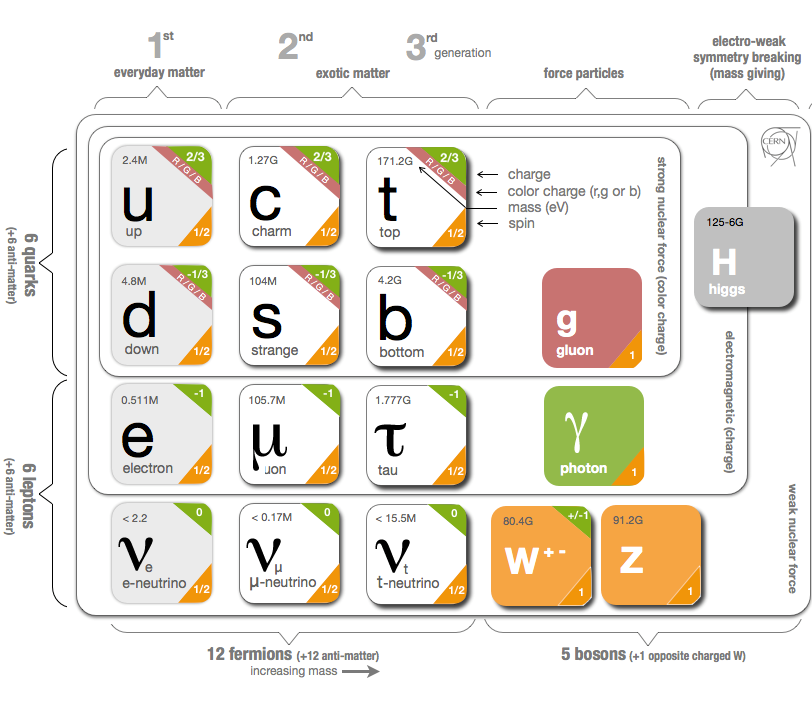
\includegraphics[width=0.90\textwidth]{../figs/Intro/StandardModel.png}}
    \caption{Standard Model Particles and Interations. Source of the figure: \cite{ref_fig_SM}.}
    \label{fig:SMtable}
  \end{center}
\end{figure}






%\subsection{Electroweak Interactions}
\label{sec:Intro_Electroweak}

\begin{figure}[htb]
  \begin{center}
    {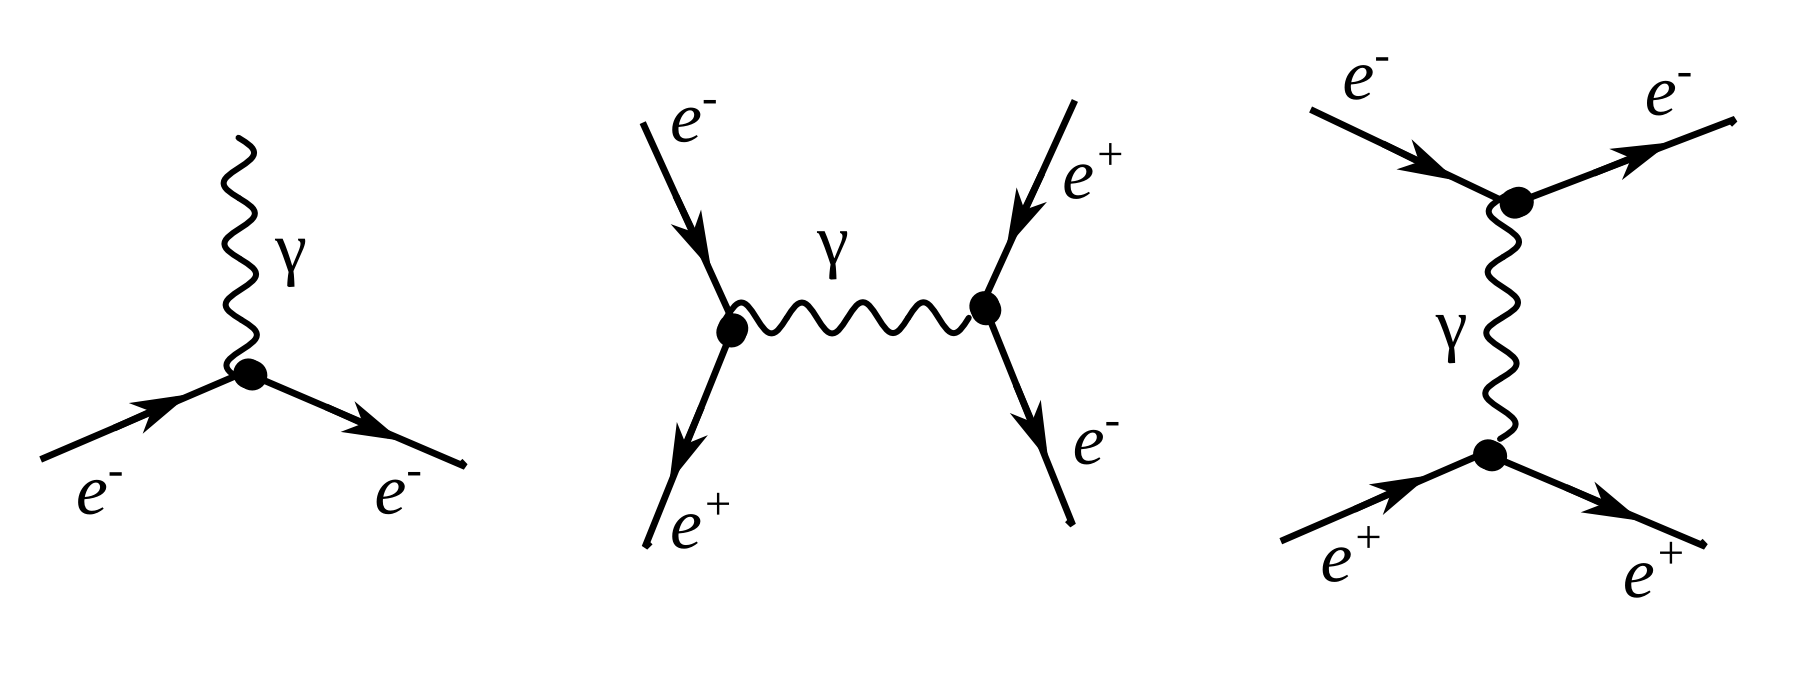
\includegraphics[width=0.90\textwidth]{../figs/Intro/feynmEM.png}}
    \caption{Electromagnetic interations}
    \label{fig:feynmEM}
  \end{center}
\end{figure}

\begin{figure}[htb]
  \begin{center}
    {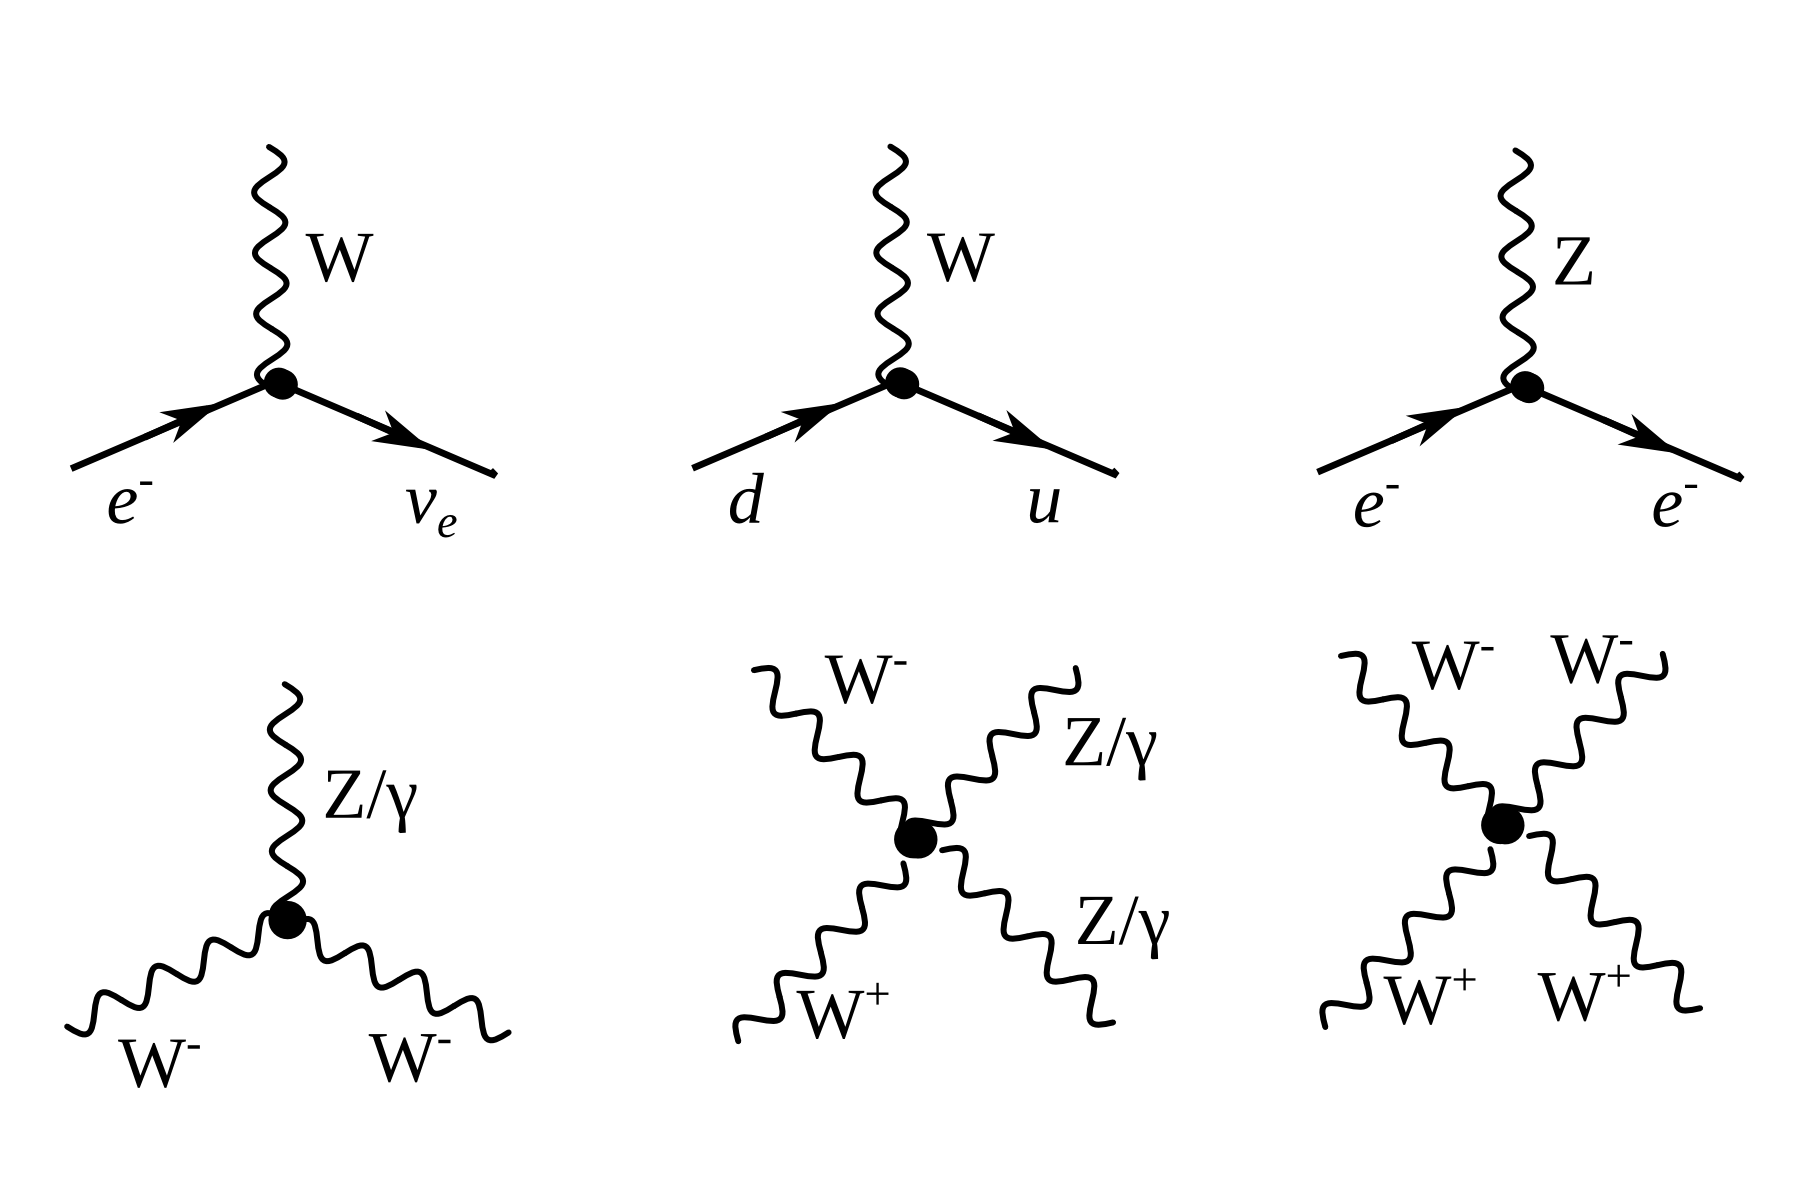
\includegraphics[width=0.90\textwidth]{../figs/Intro/feynmW.png}}
    \caption{Weak interations}
    \label{fig:feynmW}
  \end{center}
\end{figure}

All electrically charged particles participate in electromagnetic interactions. Photon, the mediator of the electromagnetic interactions, is a spin-one electrically neutral massless particle. All electromagnetic interactions can be reduced to one elementary process (Fig. \ref{fig:feynmEM}, left). This process reads: an electron enters, radiates or absorbs a photon, and escapes. Although there is an electron is drawn in this figure, it can be any other charged fermion as well. Such elementary process itself is forbidden by the energy conservation law but this element is a base of actual process (for example, Fig. \ref{fig:feynmEM}, middle and right). Such graphical representations of the particle physics processes are called Feynman diagrams. 

As for the weak interactions, there are two kinds of them: neutral (mediated by a Z boson) and charged (mediated by a W boson). Elementary processes with W and Z bosons are shown in Fig. \ref{fig:feynmW}. An electric charge must be conserved at any vertex. Therefore, if a charged lepton enters and radiates a W boson, a neutrino or antineutrino escapes (top left in Fig. \ref{fig:feynmW}). That is how a W boson interacts with a charged lepton and a neutrino. A lepton flavor number is always conserved in this interaction (Tab. \ref{tab:LeptonFlavorNumber}). 

 \begin{table}[h]
  \begin{center}
  \caption{ Lepton Flavor Number}
  \begin{tabular}{|c|c|c|c|}
     particles & $L_e$ & $L_{\mu}$ & $L_{\tau}$ \\ \hline
     $e^-,\nu_e$ &  +1  &  0  &  0  \\ \hline 
     $e^+, \bar{\nu_e}$ &  -1  &  0  &  0  \\ \hline 
     $\mu^-,\nu_{\mu}$ &  0  &  +1  &  0  \\ \hline 
     $\mu^+, \bar{\nu_{\mu}}$ &  0  &  -1  &  0  \\ \hline 
     $\tau^-,\nu_{\tau}$ &  0  &  0  &  +1  \\ \hline 
     $\tau^+, \bar{\nu_{\tau}}$ &  0  &  0  &  -1  \\ \hline 
  \end{tabular}
  \label{tab:LeptonFlavorNumber}
  \end{center}
\end{table}

From top middle diagram in Fig. \ref{fig:feynmW} we see that if a quark with Q=-1/3 enters, then a quark with Q=+2/3 escapes and, therefore, the flavor of the quarks has changed. The charged weak interaction is the only interaction which changes a quark flavor. The probability of each of three quarks with Q=+2/3 to be born is determined by the Cabibbo–Kobayashi–Maskawa matrix and is the highest for the quark of the same generation as an initial state quark (in this particular case, d is the initial state quark and u has the highest probability to be produced after an interaction with a W boson but c and t can also be produced if there is enough energy).

The right top diagram in Fig. \ref{fig:feynmW} is an emission of a Z boson off a fermion line. An electron is shown here as an example however it also could be any lepton, antilepton, quark or antiquark. All the same diagrams are possible with a photon instead of a Z boson except diagrams with neutrinos and antineutrinos.

The bottom diagrams in Fig. \ref{fig:feynmW} show self-coupling of a W boson, its interaction with Z boson and its electromagnetic radiation of a photon. WWZ, WW$\gamma$, WWZZ, WWZ$\gamma$, WW$\gamma\gamma$ and WWWW vertices are all possible in the SM.

Electromagnetic and weak interactions are unified by the electroweak theory. The mathematical formalism describing these two kinds of interactions is very similar. The difference between a photon and a Z boson is that a Z boson is massive and it can produce a neutrino-antineutrino pair or be scattered off a neutrino which a photon can not. The mass of Z boson is 91 GeV and that is why for low energies the probability of an electromagnetic process is much higher that the probability of similar neutral weak process. However, for particles with energies of E$\gg$91 GeV the mass of the Z boson can be neglected and these probabilities become the same. 

%\subsection{The Higgs Boson}
\label{Intro_Higgs}

% BAD SECTION
% NEEDS TO BE SIGNIFICANTLY REWORKED

\begin{figure}[htb]
  \begin{center}
    {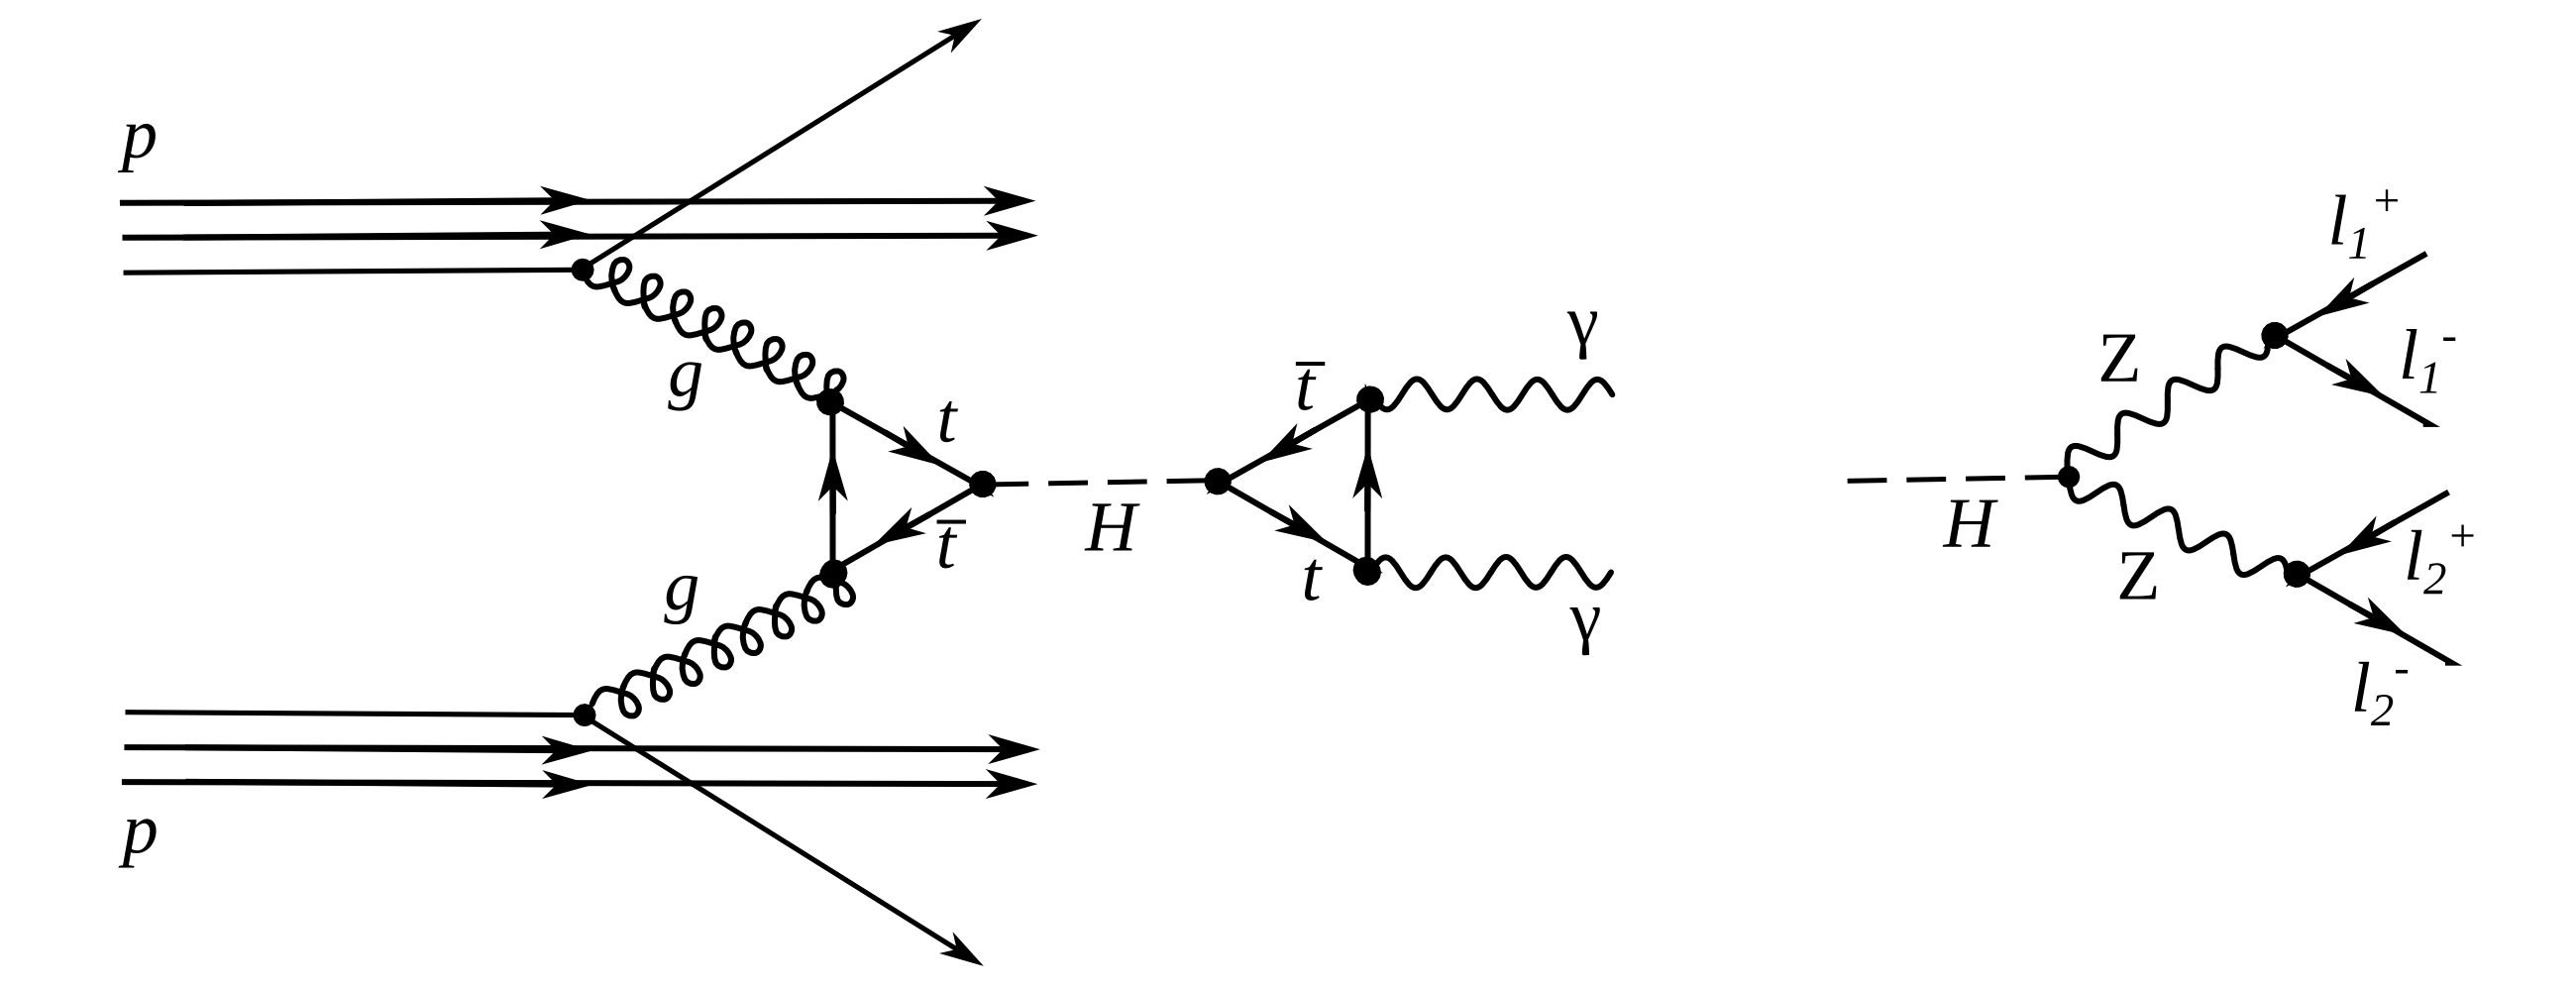
\includegraphics[width=0.95\textwidth]{../figs/Intro/FeynmanHiggs.png}}
    \caption{Higgs production and decay}
    \label{fig:higgsProduction}
  \end{center}
\end{figure}

%  I feel that there is a number of imprecise statements here that need to be corrected. Here are examples.
%   (A side note: quant is not what you mean, check the dictionary. You want to say “quantum”)
%   I would not say that the Higgs boson is a quantum of the Higgs field. The Higgs field is a doublet of complex fields, i.e. it has four components. According to wikipedia wording, for example, “it is a quantum excitation of one of the four components of the Higgs field. "
% This part: "discovered by ATLAS and CMS collaborations in the reaction shown in Fig. 4 in γγ and ZZ decay channels”
% The diagram in Fig. 4 is not appropriate for ZZ.
% "the same approach can be used to introduced masses of all elementary particles.” - but what about neutrinos? I am not sure if our favorite explanation of neutrino masses is the Higgs.
% It is not intuitive to me that larger mass means stronger interaction with the Higgs field,
% I am not sure why you say that.
% "that is how is gets its inertia”: consider rephrasing.









%\subsection{Strong Interactions}
\label{sec:Intro_QCD}

\begin{figure}[htb]
  \begin{center}
    {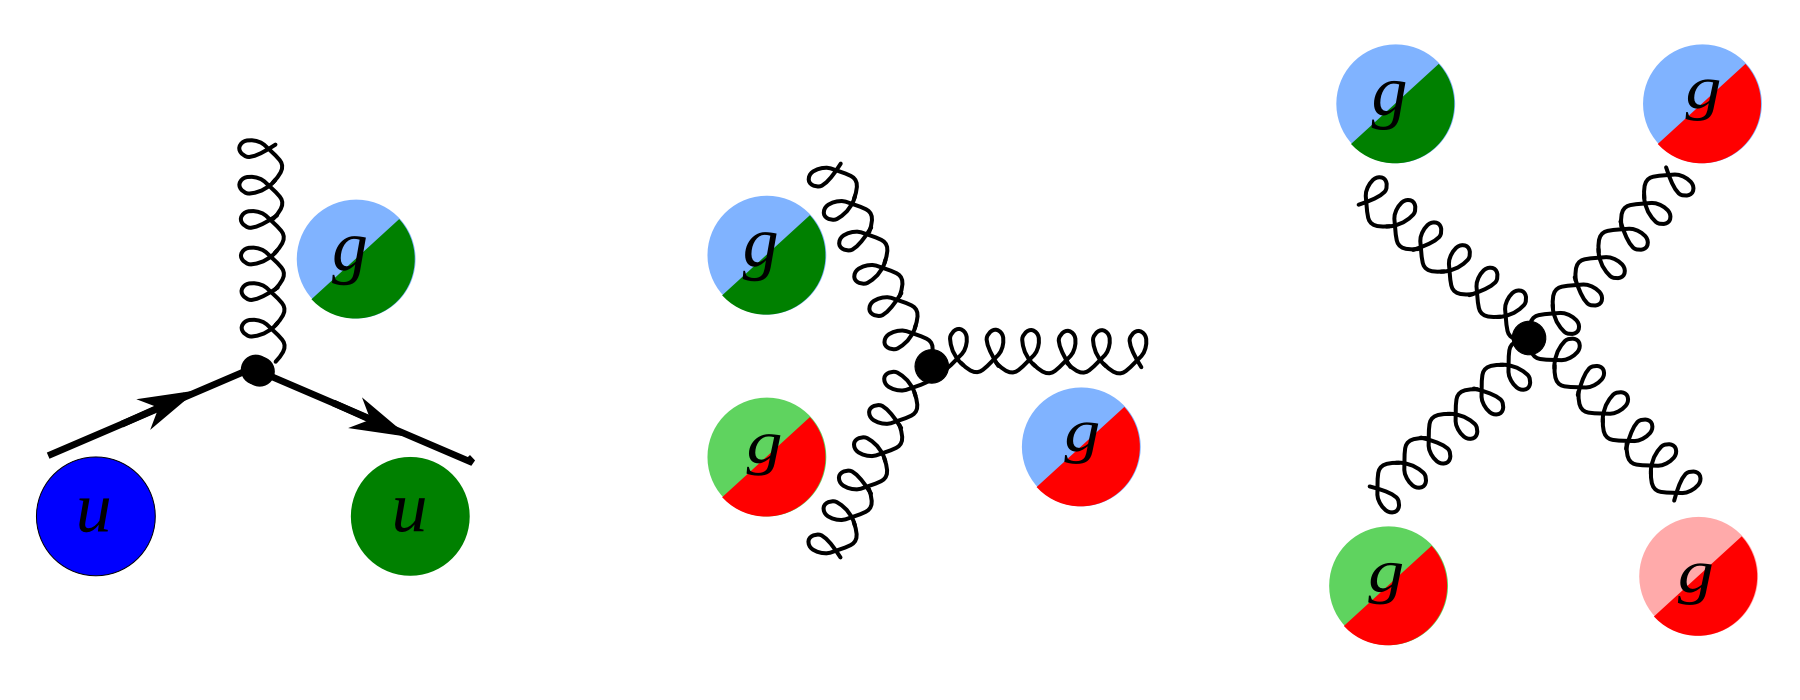
\includegraphics[width=0.80\textwidth]{../figs/Intro/feynmStrong.png}}
    \caption{Elementary processes of strong interations}
    \label{fig:feynmStrong}
  \end{center}
\end{figure}


The third fundamental force after the electromagnetic and weak ones is the strong force. The strong force is responsible for glueing protons and neutrons together in the nuclei as well as for forming protons and neutrons themselves. The strong interactions occur by exchanging gluons which are spin-one massless electrically neutral particles.  \\

The elementary strong processes are shown in Fig. \ref{fig:feynmStrong}. There are three elementary processes: $qqg$, $ggg$ and $gggg$, all are involving particles with color charges. Thus, gluons couple to quarks and self-couple. Color charges must be conserved at each elementary process of the strong interaction. Each quark possesses one of three colors at a time, and there are eight types of gluons to cover all possible color exchanges. \\

The coupling constant of the strong interaction depends on a distance between interacting particles: it becomes larger as the distance becomes larger and smaller as the distance becomes smaller. As the distance approaches zero, the coupling constant approaches zero too, and, thus, in the asymptotic limit two quarks located at the same place do not interact. This property is called asymptotic freedom.\\

On the other hand, when the distance between quarks becomes larger, the coupling constant also becomes larger. This property confines quarks to always stay in the color neutral combinations (hadrons), it forbids the existence of free quarks. A combination becomes color neutral when there is the same amount of color and anticolor or if there is the same amount of each of the three colors.  Thus, mesons are comprised of a quark and an antiquark with the opposite color charges, and baryons are comprised of three quarks: red, green and blue one. Examples of baryons include such well-known particles as a proton and a neutron.\\

The asymptotic freedom and the confinment are properties that are specific for strong interactions. The theory of strong interactions is called the QCD which is a quantum field theory invariant under $SU(3)$ color transformations. When the coupling constant is much less than one $\alpha_s \ll 1$, the perturbative approach can be used to compute observables.\\

The W$\gamma$ process being measured in this dissertation is not intended to test QCD, but a good understanding of QCD is essential for performing this measurement because the QCD corrections to the Feynman diagrams of the process are large and has to be taken into account in producing simulation. In addition, QCD describes the dynamics of quarks and gluons within colliding protons and predicts probabilities of one or another quark-antiquark pair to interact. Physics of proton-proton collisions is discussed in the subsection \ref{sec:Intro_ppCollisions}. \\

% Possible QCD corrections include quark-gluon loops at any of three quark lines as well as exchanges of gluons between different quark lines. 

%\section{Physics of Proton-Proton Collisions}
\label{sec:Intro_ppCollisions}

Consider a $pp$ collision at LHC. The proton energies are so high that each proton behaves as a complex structure. A proton is a baryon, it consists of three quarks: $uud$. These three quarks are called valence quarks. They interact with each other by exchanging gluons which produce virtual $q\bar{q}$ pairs (Fig.~\ref{fig:ppCollision}). Such virtual quarks are also called sea quarks. 

Any parton, quark, antiquark or gluon, from one proton can interact with any parton from another proton. Probabilities $f_i(x,Q^2)$ of any particular constituent $i$ to interact are described partially by QCD and partially by experimental measurements and depend on the momentum transfer $Q$ and the momentum fraction of a specific parton $x$. These probabilities are called parton distribution functions (PDFs).

\begin{figure}[htb]
  \begin{center}
    {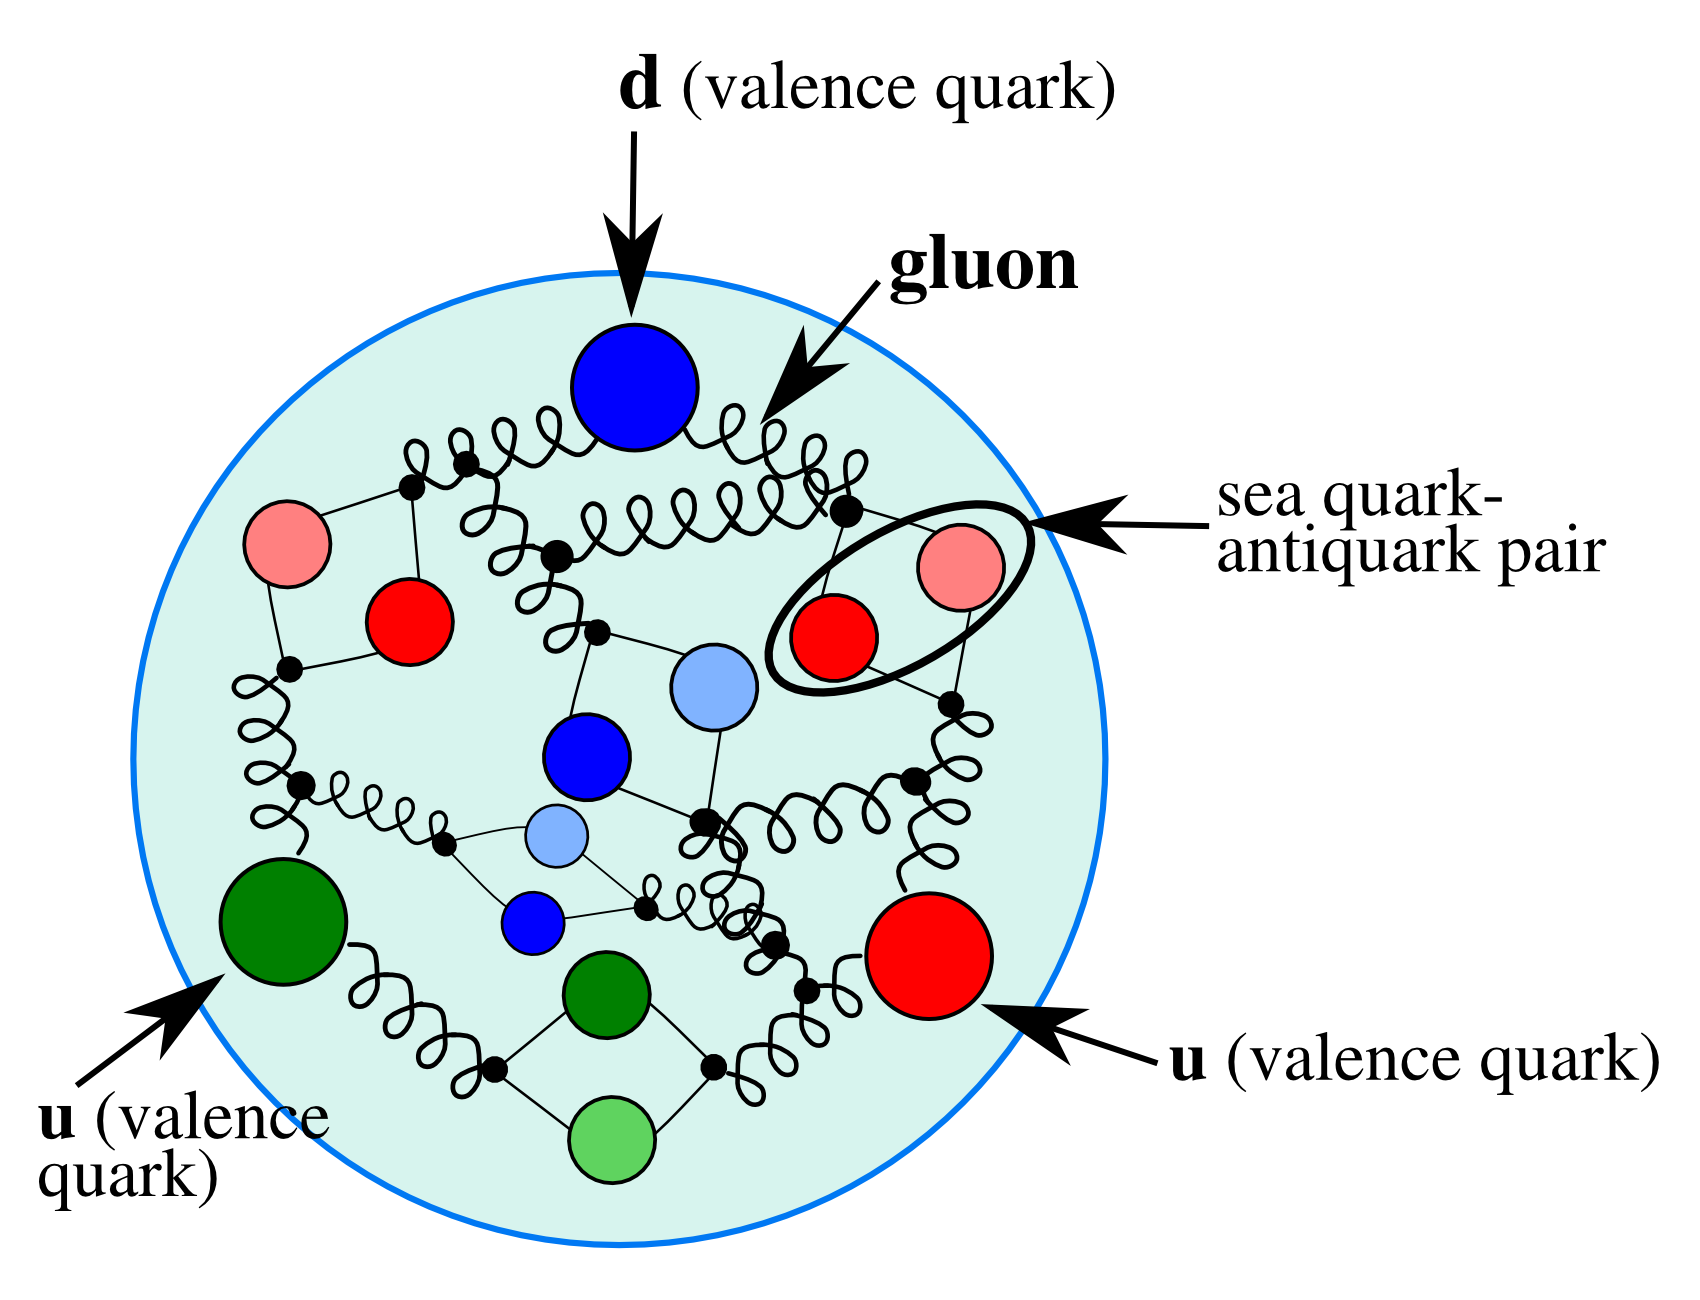
\includegraphics[width=0.45\textwidth]{../figs/Intro/protonStructure.png}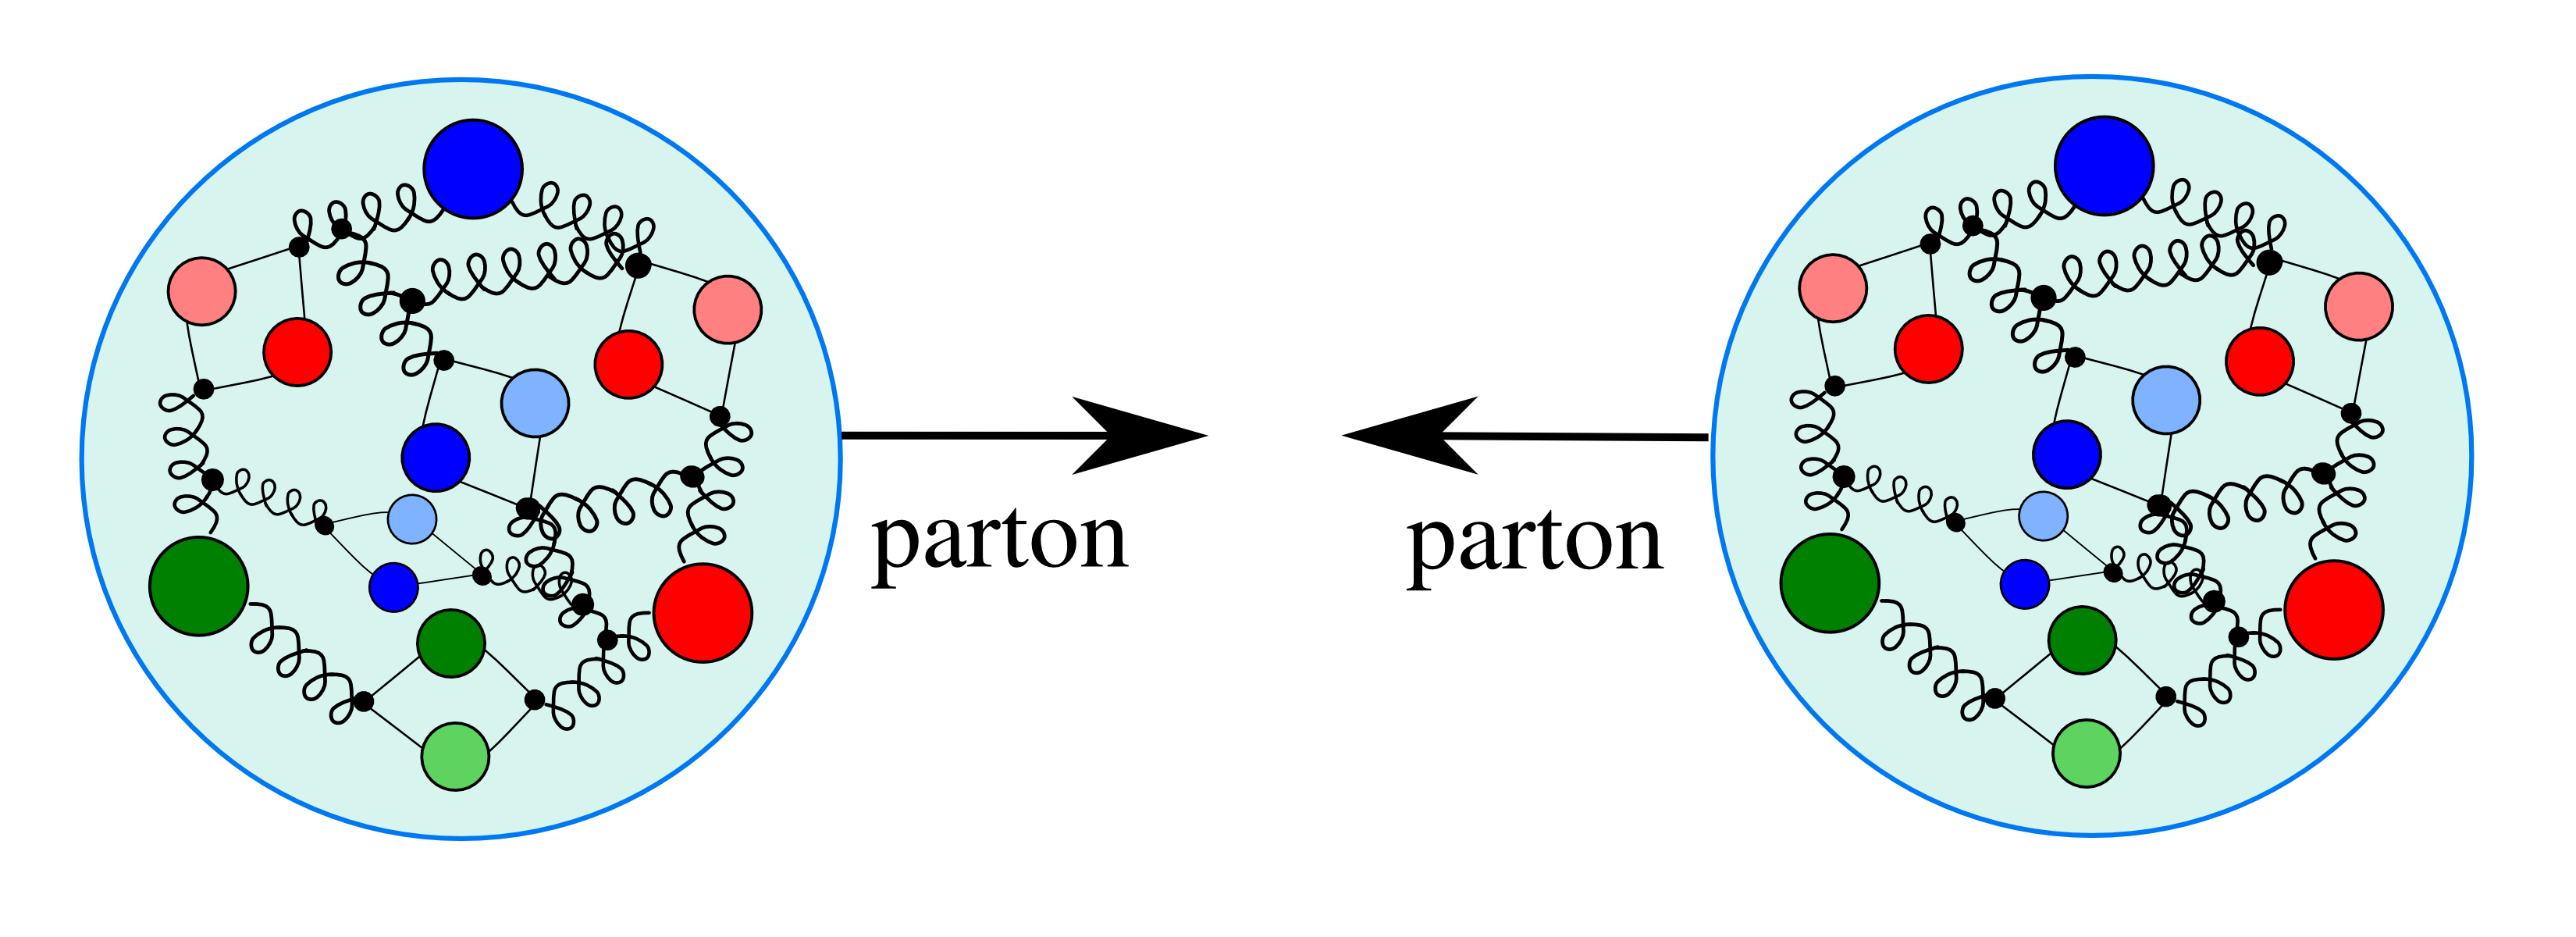
\includegraphics[width=0.45\textwidth]{../figs/Intro/ppCollision.png}}
    \caption{The proton structure (left) and the proton-proton collision (right).}
    \label{fig:ppCollision}
  \end{center}
\end{figure}

\begin{figure}[htb]
  \begin{center}
    {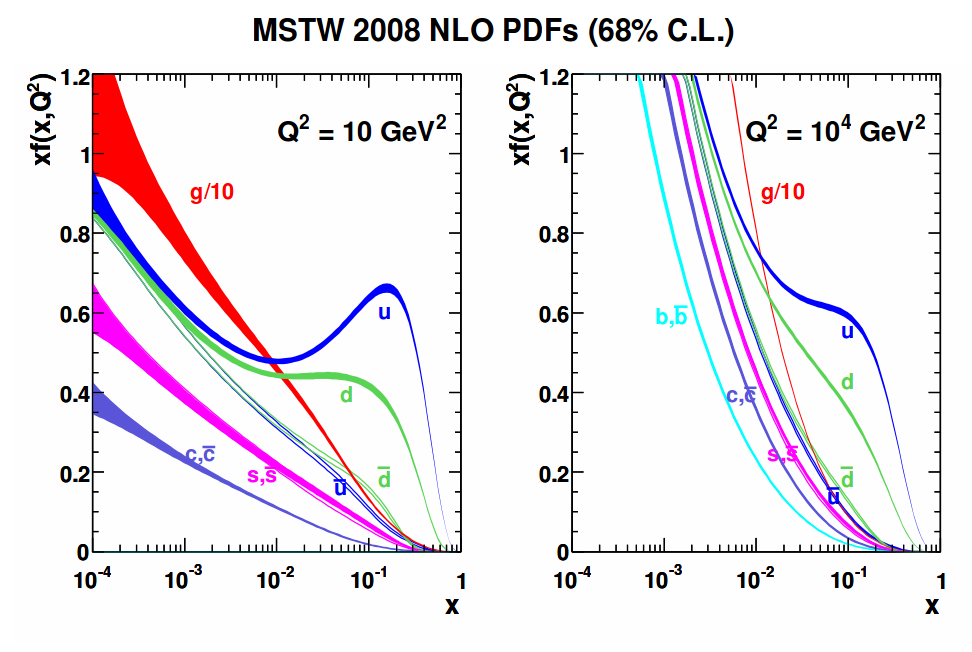
\includegraphics[width=0.85\textwidth]{../figs/Intro/pdfs.png}}
    \caption{Parton distribution functions~\cite{ref_PDG}.}
    \label{fig:pdfs}
  \end{center}
\end{figure}

For large $Q^2$ and $x$ gluon-gluon interactions have the largest probabilities to occur (Fig.~\ref{fig:pdfs}). However, gluons do not couple directly to a $W$ boson, thus, in the $W\gamma$ measurement we are mostly interested in quark-antiquark pairs which would have a total charge corresponding to the charge of a $W$ boson ($\pm 1$). Since we have $u$ and $d$ as valence quarks and we know that the probability to couple to the same generation quark in charged weak interactions is the highest, most of the $W$ bosons are created by $u\bar{d}$ and $d\bar{u}$ pairs however other $q\bar{q'}$ combinations with the total charges of $\pm 1$ are also possible. %As we look for events containing $W\gamma$ we also have other events mimicking our process. Such background events can be produced by any pair of partons.


% ADD FIGURE WITH PDFs LIKE IN THE PRESENTATION


%\subsection{Open Questions of the Standard Model}


While the SM is an accurate description of all particle physics experimental results, there are certain phenomena which are not included into the SM. In this subsection we discuss some of them.\\

The gravitational interactions do not fit into the SM. It is the open question whether the quantum theory of gravity is possible and whether there is a mediator of the gravitational interactions. Also, it is not known why the gravitational force is so much weaker than the other forces. One possible explanation comes from a theory which predicts extra spatial dimensions beyond the three we experience (e.g. the string theory). In this case, it is possible that the gravitational force is shared with other dimensions and only a fraction is available in our three dimensions.\\

Another mystery of the universe is its composition: it is known from the studies of the gravitational effects that our universe consists of dark energy by 68\%, of dark matter by 27\% and of baryon matter only by 5\%~\cite{ref_NASA}. The dark energy resists the gravitational attraction and accelerates the expansion of the universe, and is not detectable by any effects except gravitational. The understanding of dark energy is a question of general relativity rather than particle physics. The dark matter, however, likely consists of particles and therefore is a subject of particle physics. It does not radiate and that is why it cannot be detected by telescopes. The nature of the dark matter is not known but its constituents must be very stable to remain since the Big Bang. The theory of the supersymmetry which is unifying fundamental particles and mediators predicts many of new heavy particles and the lightest supersymmetric particle, the neutralino, is a good candidate for dark matter.\\

One more open question is the reason for the matter/antimatter asymmetry. Matter and antimatter should have been created in the same amount at the moment of the Big Bang. Most of it has annihilated but because of asymmetry, there was more matter than antimatter which led to the state of the Universe we observe now. There is a phenomenon of the CP-violation in weak interactions observed and described which predicts the asymmetry at a certain level. However, the effect of the CP-violation is not large enough to account for the observed amount of the matter and, therefore, the total matter/antimatter asymmetry remains unexplained. \\

The measurement of the photon transverse momentum spectrum ($P_T^{\gamma}$) of the $W\gamma$ process has a goal to both test the SM and search for the BSM physics. The low $P_T^{\gamma}$ region is not expected to be affected by any new physics and must agree well with the SM predictions while the high $P_T^{\gamma}$ region may indicate an existence of new physics if there is an enhancement over the SM predictions. The excess would be indirect evidence of the BSM particles like supersymmetric particles or additional gauge bosons which could be part of the explanation of the dark matter presence or difference in magnitudes of different interactions. More theoretical details about the SM description of W$\gamma$ process as well as possible BSM physics are given in Ch.~\ref{sec:WgAbout}. \\   

%Grand unification and super unification


